\chapter{Opis zastosowanej metody i implementacji}
\label{cha:chapter002}

\section{Opis zastosowanej metody}

\subsection{Ogólny schemat systemu}

System \textbf{mnist-translator} działa w dwóch trybach: trenowania offline
i wnioskowania (offline z CSV lub na żywo z kamery). Oba tryby korzystają
z identycznego potoku ekstrakcji cech, co gwarantuje spójność przestrzeni cech. Schemat architektury systemu wykorzystany w projekcie znajduje się w katalogu
\texttt{diagrams} i został przedstawiony na rysunku~\ref{fig:system_diagram}.

\begin{figure}[H]
    \centering
    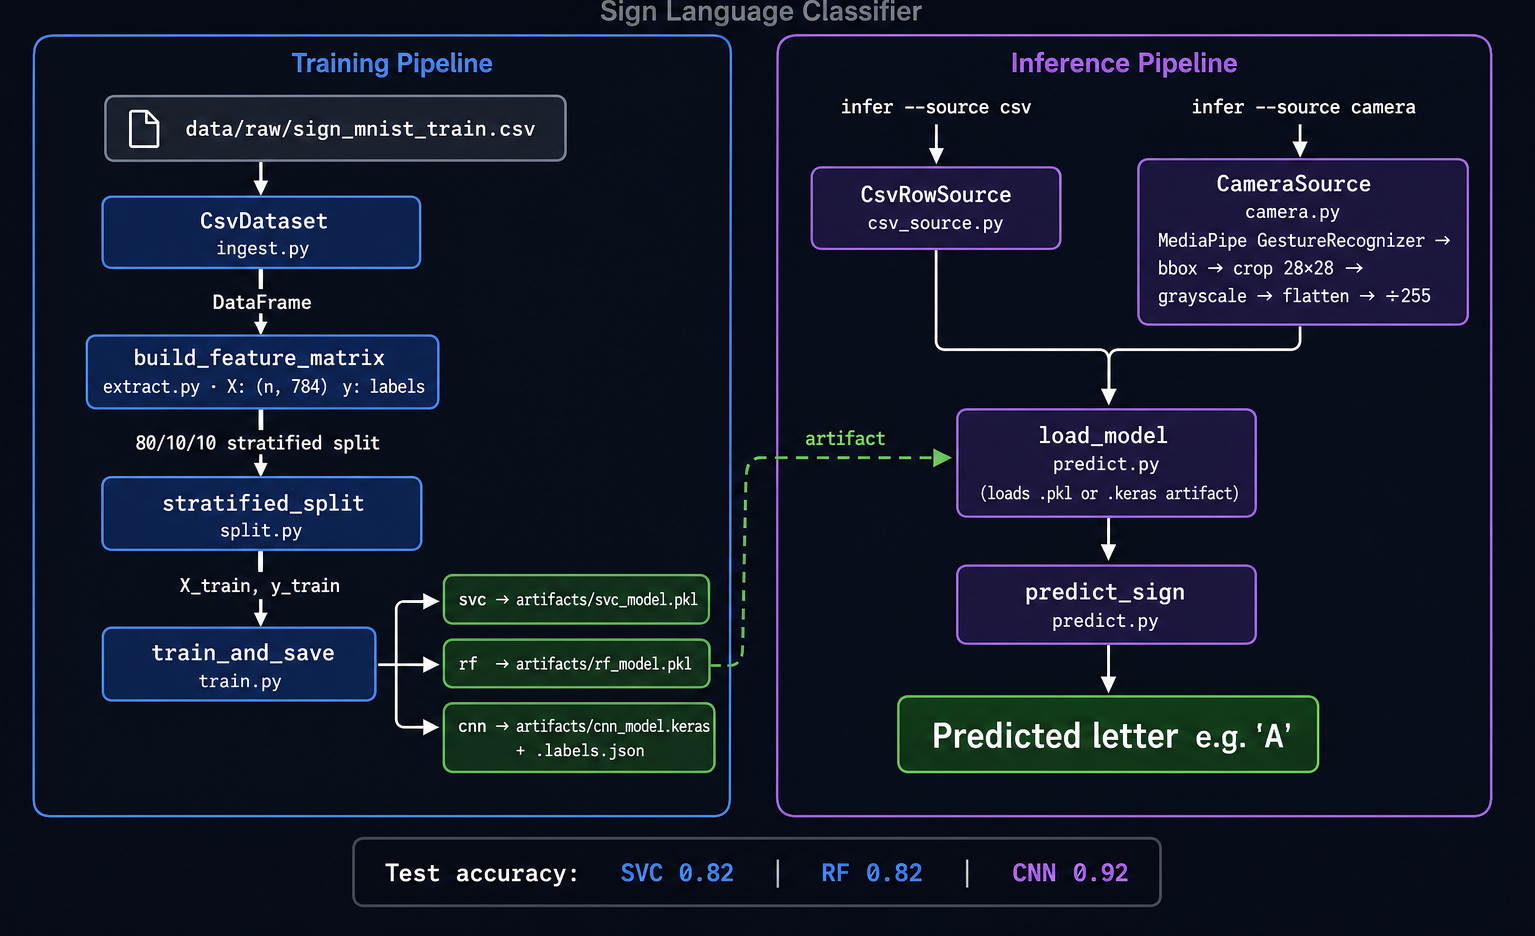
\includegraphics[width=\linewidth]{../../diagrams/architecture.png}
    \caption{Schemat systemu mnist-translator}
    \label{fig:system_diagram}
\end{figure}


\subsection{Potok przetwarzania danych}

Dane przepływają przez następujące moduły:

\begin{enumerate}
    \item \textbf{Ingestion} (\texttt{src/data/ingest.py}) --- wczytanie pliku
          CSV do struktury DataFrame i normalizacja pikseli do $[0, 1]$.
    \item \textbf{Ekstrakcja cech} (\texttt{src/data/extract.py}) --- budowa
          macierzy cech $\mathbf{X}$ (784 kolumny) i wektora etykiet $\mathbf{y}$.
    \item \textbf{Podział danych} (\texttt{src/data/split.py}) --- stratyfikowany
          podział 80/10/10 na zbiory treningowy, walidacyjny i testowy.
    \item \textbf{Trenowanie} (\texttt{src/model/train.py}) --- dopasowanie
          wybranego klasyfikatora i zapis artefaktu do katalogu \texttt{artifacts/}.
    \item \textbf{Ewaluacja} (\texttt{src/model/evaluate.py}) --- wyznaczenie
          dokładności globalnej i raportu per-klasa.
    \item \textbf{Inferencja} (\texttt{src/inference/}) --- wczytanie modelu
          i klasyfikacja nowego wektora cech.
\end{enumerate}

\subsection{Warunki pomiarowe przy inferowaniu z kamery}

Jakość predykcji w trybie kamerowym jest wrażliwa na warunki otoczenia.
Tabela~\ref{tab:warunki} zestawia zalecane ustawienia.

\begin{table}[H]
    \centering
    \caption{Zalecane warunki podczas inferencji z kamery}
    \label{tab:warunki}
    \begin{tabular}{ll}
        \toprule
        \textbf{Parametr} & \textbf{Zalecana wartość} \\
        \midrule
        Oświetlenie   & Równomierne, bez twardych cieni na dłoni \\
        Dłoń          & Lewa, skierowana przodem do kamery \\
        Kamera        & DroidCam lub dowolna obsługiwana przez OpenCV \\
        Tryb lustra   & \textbf{Wyłączony} w aplikacji kamery \\
        Tło           & Jednolity, kontrastowy kolor \\
        \bottomrule
    \end{tabular}
\end{table}

\section{Opis implementacji}

\subsection{Struktura projektu}

\begin{lstlisting}[style=styleBash, caption={Struktura katalogów projektu mnist-translator}, label=lst:struktura, numbers=none]
mnist-translator/
|-- main.py                  # Punkt wejscia CLI (brak logiki biznesowej)
|-- pyproject.toml           # Zarzadzanie zaleznosci (uv)
|-- src/
|   |-- data/
|   |   |-- ingest.py        # Ladowanie CSV i normalizacja pikseli
|   |   |-- extract.py       # Budowa macierzy cech X i etykiet y
|   |   |-- split.py         # Stratyfikowany podzial 80/10/10
|   |   `-- protocol.py      # Protokol DatasetSource
|   |-- model/
|   |   |-- train.py         # Trenowanie + zapis artefaktu
|   |   |-- evaluate.py      # Obliczanie metryk dokladnosci
|   |   `-- classifiers/
|   |       |-- svc.py       # Klasyfikator SVC z jadrem RBF
|   |       |-- random_forest.py  # Las Losowy (200 drzew)
|   |       `-- cnn.py       # Konwolucyjna siec neuronowa
|   `-- inference/
|       |-- camera.py        # Przechwytywanie wideo + MediaPipe
|       |-- csv_source.py    # Zrodlo cech z wiersza CSV
|       |-- predict.py       # Ladowanie modelu i predykcja
|       `-- protocol.py      # Protokol FeatureSource
|-- tests/                   # Testy jednostkowe (pytest)
|-- diagrams/                # Diagram architektury
`-- artifacts/               # Wytrenowane modele (gitignored)
\end{lstlisting}

\subsection{Interfejs wiersza poleceń}

Plik \texttt{main.py} udostępnia trzy tryby działania:

\begin{table}[H]
    \centering
    \caption{Tryby działania aplikacji mnist-translator}
    \label{tab:tryby}
    \begin{tabularx}{\textwidth}{llX}
        \toprule
        \textbf{Tryb} & \textbf{Opis} & \textbf{Kluczowe opcje} \\
        \midrule
        \texttt{train}  & Trenuje klasyfikator i zapisuje artefakt
                        & \texttt{-{}-classifier \{svc,rf,cnn\}}, \texttt{-{}-model}, \texttt{-{}-dataset} \\
        \texttt{eval}   & Ewaluuje model na zbiorze testowym
                        & \texttt{-{}-model}, \texttt{-{}-dataset} \\
        \texttt{infer}  & Inferencja z CSV lub z kamery
                        & \texttt{-{}-source \{csv,camera\}}, \texttt{-{}-row}, \texttt{-{}-camera} \\
        \bottomrule
    \end{tabularx}
\end{table}

\subsection{Implementacja klasyfikatorów}

\subsubsection{SVC z jądrem RBF}

\begin{lstlisting}[style=stylePython, caption={Budowa potoku SVC (src/model/classifiers/svc.py)}, label=lst:svc]
from sklearn.svm import SVC
from sklearn.pipeline import Pipeline
from sklearn.preprocessing import StandardScaler

def build_svc() -> Pipeline:
    """Buduje potok: standaryzacja + SVC z jadrem RBF."""
    return Pipeline([
        ("scaler", StandardScaler()),
        ("svc", SVC(kernel="rbf", C=10, gamma="scale",
                    decision_function_shape="ovr")),
    ])
\end{lstlisting}

\subsubsection{Las Losowy}

\begin{lstlisting}[style=stylePython, caption={Budowa Lasu Losowego (src/model/classifiers/random\_forest.py)}, label=lst:rf]
from sklearn.ensemble import RandomForestClassifier

def build_random_forest() -> RandomForestClassifier:
    """200 drzew, tryb OOB wlaczony."""
    return RandomForestClassifier(
        n_estimators=200,
        random_state=42,
        oob_score=True,
        n_jobs=-1,
    )
\end{lstlisting}

\newpage
\subsubsection{Konwolucyjna sieć neuronowa}

\begin{lstlisting}[style=stylePython, caption={Architektura CNN (src/model/classifiers/cnn.py)}, label=lst:cnn]
import tensorflow as tf

def build_cnn(num_classes: int = 24) -> tf.keras.Model:
    """Dwa bloki Conv2D->MaxPool + warstwa wyjsciowa z softmax."""
    model = tf.keras.Sequential([
        tf.keras.layers.Input(shape=(28, 28, 1)),
        tf.keras.layers.Conv2D(32, (3, 3), activation="relu",
                               padding="same"),
        tf.keras.layers.MaxPooling2D(),
        tf.keras.layers.Conv2D(64, (3, 3), activation="relu",
                               padding="same"),
        tf.keras.layers.MaxPooling2D(),
        tf.keras.layers.Flatten(),
        tf.keras.layers.Dense(128, activation="relu"),
        tf.keras.layers.Dropout(0.3),
        tf.keras.layers.Dense(num_classes, activation="softmax"),
    ])
    model.compile(optimizer="adam",
                  loss="sparse_categorical_crossentropy",
                  metrics=["accuracy"])
    return model
\end{lstlisting}

\subsection{Serializacja modeli}

Modele scikit-learn są zapisywane i wczytywane za pomocą biblioteki \texttt{joblib}:

\begin{lstlisting}[style=stylePython, caption={Zapis i odczyt modelu scikit-learn}, label=lst:joblib]
import joblib

# Zapis modelu
joblib.dump(model, "artifacts/svc_model.pkl")

# Wczytanie modelu
model = joblib.load("artifacts/svc_model.pkl")
\end{lstlisting}

Model CNN jest zapisywany w formacie natywnym Keras (rozszerzenie \texttt{.keras}):

\begin{lstlisting}[style=stylePython, caption={Zapis i odczyt modelu CNN (Keras)}, label=lst:keras]
# Zapis
model.save("artifacts/cnn_model.keras")

# Wczytanie
import tensorflow as tf
model = tf.keras.models.load_model("artifacts/cnn_model.keras")
\end{lstlisting}

\subsection{Główne zależności}

\begin{table}[H]
    \centering
    \caption{Główne zależności projektu (pyproject.toml)}
    \label{tab:deps}
    \begin{tabular}{ll}
        \toprule
        \textbf{Biblioteka} & \textbf{Zastosowanie} \\
        \midrule
        \texttt{numpy}, \texttt{pandas}   & Manipulacja danymi i macierzami \\
        \texttt{scikit-learn}             & SVC, Random Forest, metryki \\
        \texttt{joblib}                   & Serializacja modeli \\
        \texttt{opencv-python}            & Przechwytywanie klatek z kamery \\
        \texttt{mediapipe}                & Detekcja dłoni i punktów kluczowych \\
        \texttt{tensorflow >= 2.21.0}     & Budowa i trenowanie CNN \\
        \bottomrule
    \end{tabular}
\end{table}

